\documentclass{templateApunte}
\usepackage{tcolorbox}

\definecolor{Violeta}{RGB}{124,0,254}
\definecolor{Verde2}{RGB}{130,254,0} % Complementario
\definecolor{Naranja2}{RGB}{254,124,0} % Triadico
\definecolor{Verde3}{RGB}{0,254,124} % Triadico

\definecolor{Amarillo}{RGB}{249,228,0}
\definecolor{Azul2}{RGB}{0,21,249} % Complementario
\definecolor{Celeste2}{RGB}{0,249,228} % Triadico
\definecolor{Rosa}{RGB}{228,0,249} % Triadico

\definecolor{Naranja}{RGB}{255,175,0}
\definecolor{Azul3}{RGB}{0,80,255} % Complementario
\definecolor{Cian}{RGB}{0,255,175} % Triadico
\definecolor{Violeta2}{RGB}{175,0,255} % Triadico

\definecolor{Rojo}{RGB}{245,0,79}
\definecolor{Verde4}{RGB}{0,245,166} % Complementario
\definecolor{Verde}{RGB}{79,245,0} % Triadico
\definecolor{Azul}{RGB}{0,79,245} % Triadico

\definecolor{Celeste}{RGB}{0,191,255}
\definecolor{Salmon}{RGB}{255,0,157}

\newcommand{\newparagraph}{\par\vspace{\baselineskip}\noindent}
\newcommand{\hlcolor}[2]{{\sethlcolor{#1}\hl{#2}}}

\tcbuselibrary{skins}
\usetikzlibrary{shadings}
\newcounter{counter_comentario}
\newcounter{counter_observacion}
\tcbset{
  base/.style={
    empty,
    frame engine=path,
    colframe=white,
    sharp corners,
    %title={Comentario \thetcbcounter},
    attach boxed title to top left={yshift*=-\tcboxedtitleheight},
    boxed title style={size=minimal, top=4pt, left=4pt},
    coltitle=black,
    fonttitle=\large\it,
  }
}
\newtcolorbox{cP}[5]{%
  base,
  title={#3 \csname the#2\endcsname}, % Título personalizado #2 = nombre contador ; #3 = Título
  drop fuzzy shadow, % Sombra del cuadro de texto
  coltitle=#1,
  borderline west={3pt}{-3pt}{#4}, % Borde Izquierdo #4 = color del borde
  attach boxed title to top left={xshift=-3mm, yshift*=-\tcboxedtitleheight/2},
  boxed title style={right=3pt, bottom=3pt, overlay={
    \draw[draw=#5, fill=#5, line join=round]
      (frame.south west) -- (frame.north west) -- (frame.north east) --
      (frame.south east) -- ++(-2pt, 0) -- ++(-2pt, -4pt) --
      ++(-2pt, 4pt) -- cycle; % #5 = color del fondo
  }}, % Cuadro de titulo
  overlay unbroken={
    \scoped \shade[left color=#5!30!black, right color=#5]
    ([yshift=-0.2pt]title.south west) -- ([xshift=-3pt, yshift=-0.2pt]title.south-|frame.west) -- ++(0, -4pt) -- cycle;
  }, % Sombra de titulo #5 = color del titulo
  before upper={\stepcounter{#2}}
}
\newtcolorbox{cPB}[1]{%
  base,
  % drop fuzzy shadow, % Sombra del cuadro de texto
  borderline west={3pt}{-3pt}{#1}, % Borde Izquierdo #4 = color del borde
}
\begin{document}
% Seteo de contadores a 1
\setcounter{counter_comentario}{1}
\setcounter{counter_observacion}{1}

\imagenlogoU{img/LogoElNube.png}
\linklogoU{https://github.com/MarceloPazPezo}
\linkQRDoc{https://github.com/MarceloPazPezo/MyRepo/blob/main/Icinf/Semestre-8/Inteligencia-Artificial/Evaluacion-1/Evaluacion_1.pdf}
\titulo{Evaluación 1}
\asignatura{Inteligencia Artificial}
\autor{
Marcelo Paz
}
\vDoc{1.0.2}
\tipoDoc{Apunte}

% Metadatos del PDF
\title{[\asignatura]-\titulo}
\author{
    \autor
}
\portada
\margenes % Crear márgenes

\begin{abstract}
    En el siguiente documento se presenta un apunte hecho en ultimo minuto para plasmar parte de las ideas y reorganizar a mi gusto los contenidos. 
    \begin{cPB}{Azul}
      \textbf{Contenidos:}
        \begin{itemize}
            \item \hyperlink{python}{Notebook de Jupyter.}
            \begin{itemize}
              \item \hyperlink{pythonLibrerias}{Conociendo Python.}
              \item \hyperlink{algebra}{Algebra Lineal y probabilidad aplicada a IA.}
              \item \hyperlink{tcl}{Teorema Central Límite (parte teórica que guarda relación con los casos de uso del teorema).}
            \end{itemize}
            \item \hyperlink{ppt}{Presentación que contiene los conceptos de introducción a la IA.}
            \item \hyperlink{libro}{Libro Mathematics for Machine Learning (MML), pág. 17-27.}
        \end{itemize}
    \end{cPB}
\end{abstract}

\section{Inteligencia Artificial} \hypertarget{ppt}{}
Resumen:
\begin{itemize}
  \item \textbf{Objetivo:} Desarrollar algoritmos que permitan aprender de la experiencia y mejorar su rendimiento en tareas especificas, mediante la obtención de datos.
  \item \textbf{Tipos:}
  \begin{itemize}
    \item IA fuerte: Realizar tareas complejas asociadas al pensar humano (Capacidad de comprender, razonar y tomar decisiones).
    \item IA débil: Realizar tareas específicas.
  \end{itemize}
  \item Inteligencia Artificial $>$ Machine Learning $>$ Deep Learning.
  \item \textbf{Tipos de aprendizaje}
  \begin{itemize}
    \item \textbf{Aprendizaje supervisado:} En este modelo, el sistema de IA se entrena con un conjunto de datos etiquetados, es decir, datos que ya tienen la respuesta correcta. El objetivo es que el sistema aprenda a predecir la salida correcta para nuevas entradas basándose en los ejemplos proporcionados. Es útil para tareas como la clasificación de imágenes y el reconocimiento de voz.
    \item \textbf{Aprendizaje no supervisado:} A diferencia del aprendizaje supervisado, en este modelo el sistema trabaja con datos que no están etiquetados. El objetivo es encontrar patrones o estructuras ocultas en los datos. Un ejemplo común es el análisis de agrupamiento (clustering), donde el sistema agrupa datos similares sin conocer las etiquetas de antemano.
    \item \textbf{Aprendizaje por refuerzo:} En este modelo, el sistema aprende a tomar decisiones mediante prueba y error, recibiendo recompensas o castigos según el resultado de sus acciones. Es especialmente útil en situaciones donde la toma de decisiones secuenciales es crucial, como en los juegos y la robótica.
  \end{itemize}
\end{itemize}

\subsection{Machine Learning} \hypertarget{libro}{}
Resumen:
\begin{itemize}
  \item \textbf{Objetivo:} Diseñar metodologías de propósito general para extraer patrones valiosos de los datos.
  \item \textbf{Definición:} Uso de algoritmos y datos para imitar la forma en que los humanos aprenden, mejorando su precisión con el tiempo.
  \item \textbf{Núcleo:}
  \begin{itemize}
    \item Datos: Los datos son la base, la materia prima.
    \begin{itemize}
      \item Objetivo: Obtener datos de calidad para que el modelo pueda aprender de ellos.
    \end{itemize}
    \item Modelo: Los modelos estan relacionados con el proceso que genera los datos.
    \begin{itemize}
      \item Objetivo: Diseñar buenos modelos que generalicen bien a datos aún no vistos (para predecir supongo). Para que el modelo \textit{aprenda} debe mejorar su rendimiento después de procesar los datos.
      \item \hlcolor{Celeste!50}{Un buen modelo puede utilizarse para predecir lo que ocurriría en el mundo real sin necesidad de realizar experimentos.}
      \item Entrenar: Utilizar los datos disponibles para optimizar algunos parámetros del modelo con respecto a una función de utilidad que evalúa lo bien que el modelo predice los datos de entrenamiento.
    \end{itemize}
    \item Aprendizaje: Forma de encontrar automáticamente patrones y estructuras en los datos optimizando los parámetros del modelo.
  \end{itemize}

  \item Algoritmo:
  \begin{enumerate}
    \item Sistema que realiza predicciones basadas en datos. (Se denomina 'predictor').
    \item Sistema que adapta algunos parámetros internos del 'predictor' para que funcione bien con datos de entradas futuros que no se han visto. (Se denomina 'entrenamiento').
  \end{enumerate}
  \item Se puede pensar en los datos como vectores, se puede pensar en un vector:
  \begin{enumerate}
    \item Como una matriz de números (un punto de vista informático).
    \item Como una flecha con una dirección y magnitud (un punto de vista físico). 
    \item Como un objeto que obedece a la suma y la escala (un punto de vista matemático).
  \end{enumerate}

  \newpage
  \begin{figure}[H]
    \centering
    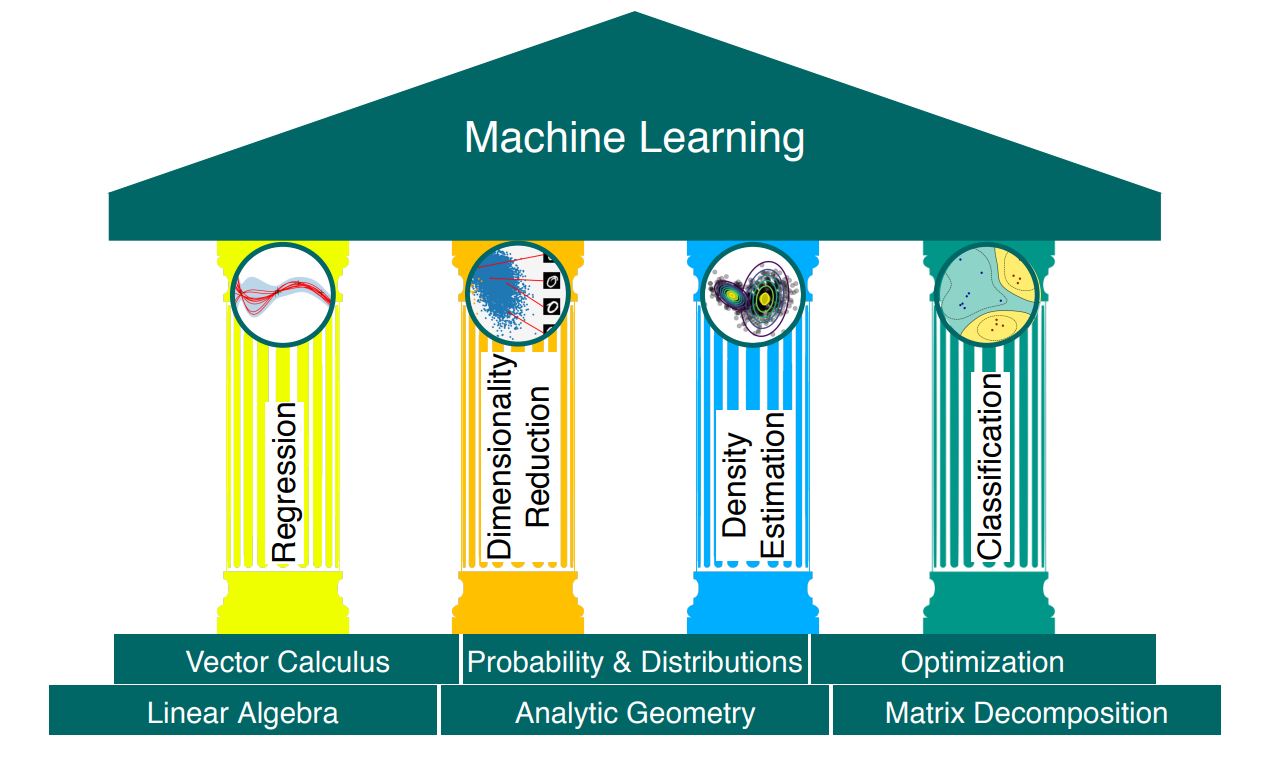
\includegraphics[width=0.75\textwidth]{img/pilaresML.png}
  \end{figure}

  \item \textbf{Pilares:}
  \begin{enumerate}
    \item \textit{Regresión:} predecir un valor continuo basado en una o más variables \newline independientes.
    \item \textit{Reducción de dimensionalidad:} reducir el número de variables en un conjunto de datos, manteniendo la mayor cantidad de información posible.
    \item \textit{Estimación de densidad:} proceso de construir una función que describe la distribución de probabilidad de una variable aleatoria.
    \item \textit{Clasificación:} asignar una etiqueta a una observación basada en uno o más atributos.
  \end{enumerate}

  \item \textbf{Bases de los pilares:}
  \begin{itemize}
    \item Nivel 1:
    \begin{itemize}
      \item \textit{Álgebra Lineal:} Representamos los datos numéricos como vectores y \newline representamos una tabla de dichos datos como una matriz. El estudio de vectores y matrices se denomina álgebra lineal
      \item \textit{Geometría Analítica:} Dado que dos vectores representan dos objetos en el mundo real, queremos hacer afirmaciones sobre su similitud. La idea es que nuestro algoritmo de aprendizaje automático (nuestro predictor) prediga que los vectores que son similares tienen resultados similares. 
      Para formalizar la idea de similitud entre vectores, necesitamos introducir operaciones que tomen dos vectores como entrada y devuelvan un valor numérico que represente su similitud. La construcción de la semejanza y las distancias es central para la geometría analítica.
      \item \textit{Descomposición de la matriz:} En el capítulo 4, introducimos algunos conceptos fundamentales sobre las matrices y la descomposición de matrices. Algunas operaciones en matrices son extremadamente útiles en el aprendizaje automático y permiten una interpretación intuitiva de los datos y un aprendizaje más eficiente.
    \end{itemize}

    \newpage
    \item Nivel 2:
    \begin{itemize}
      \item \textit{Cálculo vectorial y optimización:} Para entrenar modelos de aprendizaje automático, normalmente encontramos parámetros que maximizan alguna medida de rendimiento. Muchas técnicas de optimización requieren el concepto de gradiente, que nos indica la dirección en la que debemos buscar una solución.
      El capítulo 5 trata sobre el cálculo vectorial y detalla el concepto de cálculo vectorial de gradientes, que posteriormente utilizaremos en el capítulo 7, donde hablamos de optimización para encontrar máximos/ mínimos de funciones.
      \item \textit{Probabilidad y distribución:} A menudo consideramos que los datos son observaciones ruidosas de alguna señal subyacente verdadera. Esperamos que mediante la aplicación del Machine learning podamos identificar la señal del ruido. Esto requiere que tengamos un lenguaje para cuantificar lo que significa "ruido". A menudo también nos gustaría tener predictores que nos permitan expresar algún tipo de incertidumbre, por ejemplo, para cuantificar la confianza que tenemos sobre el valor de la predicción en un punto de datos de prueba particular. La cuantificación de la incertidumbre es el ámbito de la teoría de la probabilidad.
    \end{itemize}
  \end{itemize}
\end{itemize}

\subsection{Matemática para Machine Learning (MML)}
\begin{figure}[H]
  \centering
  \begin{overpic}[width=1\textwidth]{img/vistaGeneralConceptosMatematicos.png}
    \put(43.2,56.8){\hyperlink{vector}{\phantomsection\hspace{2.4em}\raisebox{0pt}[0.4cm][0.12cm]{}}}
    \put(27.6,43.5){\hyperlink{matriz}{\phantomsection\hspace{2.4em}\raisebox{0pt}[0.4cm][0.12cm]{}}}
    \put(3.1,30.3){\hyperlink{sistemaLineal}{\phantomsection\hspace{5.8em}\raisebox{0pt}[0.4cm][0.22cm]{}}}
    % \put(2.6,30.2){\hyperlink{sistemaLineal}{\colorbox{yellow}{\phantomsection\hspace{5.8em}\raisebox{0pt}[0.4cm][0.22cm]{}}}}
  \end{overpic}
\end{figure}

\newpage
\subsection{Python en ML} \hypertarget{python}{}
\begin{itemize}
  \item \hypertarget{pythonLibrerias}{\textbf{Librerías:}}
  \begin{itemize}
    \item \textbf{Numpy:} Librería de Python que proporciona soporte para arreglos y matrices multidimensionales, junto con una colección de funciones matemáticas de alto nivel para operar en estos arreglos.
    \item \textbf{Pandas:} Librería de Python que proporciona estructuras de datos y herramientas de análisis de datos.
    \item \textbf{Matplotlib:} Librería de Python que proporciona una API orientada a objetos para incorporar gráficos en aplicaciones usando GTK, Qt, WxWindows o Mac OS X.
    \item \textbf{Seaborn:} Librería de Python que proporciona una interfaz de alto nivel para dibujar gráficos estadísticos atractivos y informativos (basada en matplotlib).
    \item \textbf{SciPy:} Librería de Python que se utiliza para realizar cálculos científicos y técnicos (numpy con esteroides).
    \item \textbf{Scikit-learn:} Librería de Python que se usa para construir y evaluar modelos de aprendizaje automático.
  \end{itemize}

  \item Colecciones de datos:
  \begin{itemize}
    \item Tuplas ( ): Son inmutables, es decir, no se pueden modificar después de su creación.
    \item Listas [ ]: Son mutables, es decir, se pueden modificar después de su creación.
    \item Diccionarios \{ \}: Son colecciones de datos que contienen pares clave-valor.
  \end{itemize}

  \item \textbf{Tensor:} puede ser un número, un vector, una matriz o cualquier colección de estos objetos.
  \begin{itemize}
    \item Tensor grado 0: Escalar (número).
    \item Tensor grado 1: Vector.
    \item Tensor grado 2: Matriz.
    \item Tensor grado 3: 3D.
    \item Tensor grado n: nD.
  \end{itemize}
  \item \textbf{Álgebra Lineal:} \hypertarget{algebra}{}
  \begin{itemize}
    \item \hypertarget{vector}{\textbf{Vector:}} Es un conjunto de números de una sola dimensión.
    \begin{equation*}
      \vec{v} =
      \begin{pmatrix}
        v_1 \\
        v_2 \\
        v_3
      \end{pmatrix}
    \end{equation*}

    \item \hypertarget{matriz}{\textbf{Matriz:}} Es un conjunto de números de dos dimensiones.
    \begin{equation*}
      M =
      \begin{pmatrix}
        x_{11} & x_{12} & x_{13} \\
        x_{21} & x_{22} & x_{23} \\
        x_{31} & x_{32} & x_{33}
      \end{pmatrix}
    \end{equation*}

    \item Lo más relevante es:
    \begin{itemize}
      \item \textbf{Producto punto entre vectores} (Se obtiene un escalar).
      
      \item \textbf{Multiplicación de matrices} (Se obtiene una matriz).
      
      \item \textbf{Vector ortogonal:} Dos vectores son ortogonales si su producto punto es cero.
      
      \item \textbf{Matriz ortogonal:} Una matriz es ortogonal si sus columnas son ortogonales entre sí y tienen una longitud de 1.
      \begin{equation*}
        A^T \cdot A = I
      \end{equation*}

      \item \textbf{Matriz inversa:} Una matriz tiene una inversa si su determinante es diferente de cero.
      
      \item \textbf{Matriz transpuesta:} La matriz transpuesta de una matriz es una matriz que se obtiene intercambiando filas por columnas.

      \item \textbf{Vector propio:} Un vector propio (o autovector) de una matriz es un vector no nulo que cambia de magnitud pero no de dirección cuando se aplica la matriz a él.
      
      \item \textbf{Descomposición en valores singulares (SVD):} SVD es una técnica importante en la reducción de dimensionalidad y se utiliza en métodos como PCA y en el tratamiento de datos en IA.
      
      \item \hypertarget{sistemaLineal}{\textbf{Sistema de ecuaciones lineales:}} Un sistema de ecuaciones lineales es un conjunto de ecuaciones lineales que comparten las mismas variables.
      \begin{equation*}
        Ax = b
      \end{equation*}
      Donde:
      \begin{itemize}
        \item $A$ es una matriz de coeficientes.
        \item $x$ es un vector de incógnitas.
        \item $b$ es un vector de términos independientes.
        \item Posibles soluciones:
        \begin{enumerate}
          \item Ninguna solución: rango(A) $\neq$ rango(A,b).
          \item Infinitas soluciones: rango(A) = rango(A,b) $<$ n.
          \item Solución única: rango(A) = rango(A,b) = n.
        \end{enumerate}
      \end{itemize}
    \end{itemize}
  \end{itemize}
  \item \textbf{Probabilidad:}
  \begin{itemize}
    \item \textbf{Distribución normal:} Es una distribución de probabilidad continua que se utiliza para representar variables aleatorias con distribuciones simétricas alrededor de su media. Se utiliza en técnicas de regresión y modelos probabilísticos.
    \item \textbf{Teorema de Bayes:} Se utiliza en métodos de clasificación como el clasificador Naive Bayes y en la inferencia probabilística en redes bayesianas.
    
    \newpage
    \item \hypertarget{tcl}{\textbf{Teorema central del límite:}} Es un teorema fundamental en estadística que establece que, a medida que el tamaño de la muestra aumenta, la distribución de la media de la muestra se aproxima a una distribución normal.
    \begin{itemize}
      \item \textbf{Aplicaciones:}
      \begin{itemize}
        \item \hlcolor{Celeste!50}{Justificación para la inferencia estadística.}
        \begin{enumerate}
          \item \hlcolor{Verde3!80}{Modelos de regresión y clasificación: En la mayoría de los algoritmos de aprendizaje supervisado,} como la regresión lineal, logística y otros métodos basados en gradiente, \hlcolor{Verde3!80}{se supone que los errores (residuos) tienen una distribución normal. El TCL proporciona una justificación teórica para esta suposición cuando el tamaño de la muestra es grande.}
          \newparagraph
          \item \hlcolor{Amarillo!80}{Intervalos de confianza y prueba de hipótesis:} En Machine Learning y Deep Learning, \hlcolor{Amarillo!80}{se realizan pruebas estadísticas para validar los modelos, y el TCL permite que los intervalos de confianza y las pruebas de hipótesis sean válidas para la mayoría de las estadísticas.}
        \end{enumerate}
        
        \item \hlcolor{Celeste!50}{Entrenamiento de redes neuronales y optimziación.}
        \begin{enumerate}
          \item \hlcolor{Verde3!80}{Inicialización de Pesos: al entrenar redes neuronales profundas, los pesos se inicializan típicamente utilizando distribuciones normales. El TCL asegura que, con un gran número de nodos y conexiones, las sumas de muchas variables aleatorias (como activaciones) tienden a ser normalmente distribuidas.} \newline Esto facilita el cálculo de las actualizaciones de los pesos utilizando métodos basados en gradientes.
          \newparagraph
          \item \hlcolor{Amarillo!50}{Propagación de Errores: en el entrenamiento de redes neuronales, los gradientes calculados a través del algoritmo de retropropagación a menudo se comportan como variables aleatorias. El TCL sugiere que la distribución de estos gradientes se aproximará a una distribución normal a medida que el tamaño de la red y la cantidad de muestras de entrenamiento aumentan, lo que estabiliza el proceso de optimización.}
        \end{enumerate}
        
        \newparagraph
        \item \hlcolor{Celeste!50}{Validación de modelos y evaluación de rendimiento.}
        \begin{enumerate}
          \item \hlcolor{Verde3!50}{Bootstraping y Métodos de Muestreo: el TCL se utiliza para justificar el uso de técnicas de remuestreo como el bootstrapping en Machine Learning. Estas técnicas permiten estimar el error y la varianza de los modelos, proporcionando distribuciones normales aproximadas de los estimadores cuando se remuestrean múltiples veces.}
          \newparagraph
          \item \hlcolor{Amarillo!50}{Curvas ROC y AUC: en la evaluación del rendimiento del modelo, las áreas bajo las curvas ROC (AUC) a menudo se aproximan a una distribución normal debido al teorema central del límite, lo que permite comparar diferentes modelos estadísticamente.}
        \end{enumerate}

        \newpage
        \item \hlcolor{Celeste!50}{Reducción de dimensionalidad y preprocesamiento de datos.}
        \begin{enumerate}
          \item \hlcolor{Verde3!80}{PCA (Análisis de Componentes Principales): cuando se reduce la dimensionalidad de los datos mediante técnicas como PCA, el TCL asegura que, para un gran número de muestras, la suma de los componentes principales tiende a una distribución normal.} \newline Esto ayuda en la selección y retención de características más relevantes y facilita el análisis y la visualización.
        \end{enumerate}

      \end{itemize}
    \end{itemize}
  \end{itemize}
\end{itemize}

\end{document}